\documentclass[a4paper,twoside]{article}

\usepackage{epsfig}
\usepackage{subfigure}
\usepackage{calc}
\usepackage{amssymb}
\usepackage{amstext}
\usepackage{amsmath}
\usepackage{amsthm}
\usepackage{multicol}
\usepackage{pslatex}
\usepackage{apalike}
\usepackage{SCITEPRESS}
\usepackage[small]{caption}
\usepackage{color}

\usepackage[Pseudocode]{algorithm}
\usepackage{algorithmic}
\renewcommand{\thealgorithm}{}

\subfigtopskip=0pt
\subfigcapskip=0pt
\subfigbottomskip=0pt

\newenvironment{courier}{\fontfamily{courier}\selectfont}{\par}

\newcommand\dotaligner{\texttt{DotAligner}}
\newcommand\pmcomp{\texttt{pmcomp}}
\newcommand\pmmulti{\texttt{pmmulti}}
\newcommand\clustgraph{\texttt{ClustGraph}}
\newcommand\locarna{\texttt{LocaRNA}}
\newcommand\rnaplfold{\texttt{RNAplfold}}
\newcommand\pvclust{\texttt{pvclust}}
\newcommand\carna{\texttt{CARNA}}
\newcommand\petfold{\texttt{PETfold}}
\newcommand\rnalocal{\texttt{RNAlocal}}
\newcommand\eg{\textit{e.g.}}
\newcommand{\RED}[1]{\textcolor{red}{#1}}

\begin{document}

\title{Clustering of common structured RNA domains by aligning basepair probabilities}

\author{\authorname{Stefan E Seemann\sup{1,2}, Martin A Smith\sup{1}}
\affiliation{\sup{1}Garvan Instistute of Medical Research, 384 Victoria Street, Sydney, NSW, Australia}
\affiliation{\sup{2}University of Copenhagen, Groennegaardsvej 3, Frederiksberg, Denmark}
\email{seemann@rth.dk}
}

\keywords{RNA secondary structure, Basepair probability, Structure-based alignment}


%at least 70 and at most 200 words
\abstract{RNA molecules often function by their RNA secondary structure. Many
short RNAs have characteristic global structures, such as the two sequential
stem-loop structures of HACA snoRNAs. Long noncoding RNAs (lncRNAs) have
important local structured RNA domains that are, for instance, recognized by RNA
binding proteins. The discovery of functional RNA domains demands fast and
accurate clustering approaches that are based on the structure landscape of RNA
sequences. The gold standard of comparative RNA analysis, namely Sankoff-style
simultaneous alignment and folding, is, however, not applicable. Here, we
present a novel algorithm for RNA structure alignments that we named \dotaligner.
The presented method optimizes the alignment of two RNA sequences with respect
to all possible structures simultaneously, which allows the alignment of similar
structured RNA domains of low sequence similarity.  The generated dissimilarity
matrices are used to cluster RNA sequences in common structured RNA domains. The
method was successfully tested on a selected set of HACA-box snoRNAs. It can
contribute to the detection of functional RNA domains through its speed and very
high specificity.}

\onecolumn \maketitle \normalsize \vfill


\section{\uppercase{Introduction}}
\label{sec:introduction}

\noindent The structure of RNA molecules is an essential functional criteria of
many non-coding RNAs (ncRNAs), such as the stem-loop of microRNAs and the double
stem-loop RNA motifs of the HOTAIR long ncRNA \cite{Gupta20393566}. NcRNAs can
be devided in RNA families of similar inherent functionality, structures, or
composition. The largest collection of RNA families is the Rfam database with
2,208 families in its version 11.0 \cite{Burge23125362}. However, high-througput
sequencing continuously uncovers novel non-coding RNA transcripts and
genome-wide RNA structure predictions have revealed hundreds of thousands
putative conserved RNA secondary structures. We hypothesize that the RNA
secondary structure is the scaffold for intermolecular interactions of many
ncRNA-driven regulatory pathways. Protein binding domains of RNA molecules may
evolve totally independent from sequence and, instead, may be solely determined
by structure. It has been shown that if the sequence similarity falls below 60\%
sequence comparison will not find anymore domain similarities that are based on
structure \cite{Gardner15860779}. In addition, competing structures and
suboptimal structures may support or even drive the functionality of an RNA
domain. Hence, methods are needed that find structural similarity independent
from sequence conservation and freed from one single optimal RNA secondary
structure.

For clustering of RNA domains a dissimilarity measurement of all pairs of query
structures is needed. The dissimilarity is described through a pairwise weighted
string alignment with arbitrary pairwise dependencies (for base pairings). The
Needleman-Wunsch (2) algorithm solves the maximum weight string alignment
problem by dynamic programming in $O(n^2)$ by preserving the sequence order and
maximizing the similarity. The consideration of pairs of nucleotides in each
sequence that form intra-molecular interactions extends the problem to pairwise
dependencies among positions in each string. This problem variant is
MAX-SNP-hard. However, the problem can be attacked by intelligent heuristics
that avoid the examination of all possible aligning states.

Simultaneous alignment and folding \cite{sankoff85} is the acknowledged gold
standard to predict the consensus structure and alignment of a set of related
RNA sequences. Because the Sankoff algorithm is practically not applicable, the
pre-calculation of the structure ensemble of each sequence, \eg{} basepair
probabilities in thermodynamically equilibrated RNA structure ensembles
\cite{McCaskill:1990}, is used by different methods to speed up the calculation
of structure-based alignments. The programs \pmcomp{} for pairwise and
\pmmulti{} for multiple alignments \cite{Hofacker15073017}, as well as
\locarna{} \cite{Will17432929} score the alignment based on the notion of a
common secondary structure. Despite of the usage of the basepair probability
matrices extract these methods the maximum-weight common secondary structure but
do not explicitely consider suboptimal structures in the alignment. The pairwise
alignment of basepair probability matrices (dot plots) has been first introduced
by \carna{} \cite{Palu2010,Sorescu2012}. \carna{} finds iterativelly better
alignments with an effective constraint programming technique using a branch and
bound scheme (propagator).

Beside of \locarna{} and a method based on directed acyclic graph kernels
\cite{Sato18647390}, the alignment-free approach \clustgraph{}
\cite{Heyne22689765} has been used to cluster RNA structure in common domains.
Here, we propose an alternative heuristic for the pairwise weighted string
alignment with arbitrary pairwise dependencies that can deliver dissimilarity
scores of dot plots in time close to an Needleman-Wunsch alignment which makes
the approach applicable for clustering of large numbers of putative RNA domains.


\section{\uppercase{Implementation}}

\noindent The proposed algorithm makes the computationally complex problem of
aligning two dotplots available by the iteration through a two step approach:
(1) find dissimilarity (distance) of basepair probabilities of each nucleotide
in sequence $S_a$ to each nucleotide in sequence $S_b$; and (2) find best path
through the distance matrix generated in 1. The iteration is stopped when no
more gaps are introduced in step 2. This algorithm runs in $O(n^2)$, hence, in
the same time complexity as the sequence-based alignments.  In the following we
discuss in detail how the algorithm works.

As described in \cite{Palu2010} the weight $Z$ of alignment \emph{A} of two
arc-annotated sequences $(S_a,P_a)$ and $(S_b,P_b)$ is defined by

\begin{equation}\label{eq1}
	Z(A) = \sum_{(i,i^\prime) \in A} \sigma(i,i^\prime) + \sum_{(i,j) \in
	P_a,\atop {(i^\prime,j^\prime) \in P_b,\atop {(i,i^\prime) \in
	A, (j,j^\prime) \in A}}} \tau(i,j,i^\prime,j^\prime) + \gamma
	\times L,
\end{equation}

where $S$ is a sequence and $P$ is a base pairing probability matrix,
$\sigma(i,i^\prime)$ is the similarity of sequence positions $S_a[i]$ and
$S_b[i^\prime]$, $\tau(i,j,i^\prime,j^\prime)$ is the similarity of arcs $(i,j)
\in P_a$ and $(i^\prime,j^\prime) \in P_b$ ($\tau(i,j,i^\prime,j^\prime) = 1 -
2 \times | P_a(i,j)-P_b(i^\prime,j^\prime) |$), and $\gamma$ is the gap cost
associated with each sequence position that is not matched ($L =
|S_a|+|S_b|-2|A|$). The alignment problem finds the maximal $Z(A)$. As its
solution is MAX-SNP-hard we implemented a heuristic of the alignment problem in
\dotaligner{} which is summarized in the following pseudocode:

%\begin{courier}Example\end{courier}
\begin{small}
\begin{algorithm}
\caption{\\ Get Alignment $A$ of the two dotplots $P_a$ and $P_b$}
%\begin{algorithmic}[1]
\begin{algorithmic}
%\begin{courier}
\REQUIRE \begin{courier}$(S_a,P_a)$ of length $N$, $(S_b,P_b)$ of length $M$\end{courier}
\REPEAT
\STATE \begin{courier}\COMMENT{STEP 1: global alignment of pairing probabilities of each base in $S_a$ and $S_b$}\end{courier}
\FOR{$i=1$ to $N$}
\FOR{$i^\prime=1$ to $M$}
\STATE {\arraycolsep=1pt
\vspace{-15px}
\begin{equation}\label{eq2}
\begin{array}{rl}
	Z(A|i,i^\prime) = & \alpha \times \sigma(i,i^\prime) + \\
%	& \beta \times \sum_{k=1}^N \sum_{l=1}^M \tau(i,k,i^\prime,l) + \\
	& \beta \times \sum_{(i,j) \in P_a,\atop {(i^\prime,j^\prime) \in P_b,\atop {(j,j^\prime) \in A}}} \tau(i,j,i^\prime,j^\prime) + \\
	& \gamma \times L
%NW[P_a(x_{i1} \ldots x_{iN}),P_b(y_{j1} \ldots y_{jM})]
\end{array}
\end{equation}}
\vspace{-10px}
\ENDFOR
\ENDFOR
\STATE \begin{courier}\COMMENT{STEP 2: local alignment of pairwise weights $Z(A|i,i^\prime)$}\end{courier}
\FOR{$i=1$ to $N$}
\FOR{$j=1$ to $M$}
\STATE
\vspace{-15px}
\begin{equation}\label{eq3}
H_{ij} = max \begin{cases}
	0 \\
	H_{i-1 j} + \gamma \\
	H_{i-1 j-1} + Z(A|i-1,j-1) \\
	H_{i j-1} + \gamma
\end{cases}
\end{equation}
\vspace{-10px}
\ENDFOR
\ENDFOR
\STATE $A(S_a,S_b) = BACKTRACKING(H)$
\STATE Remove gaps in $A(S_a,S_b)$ from $(S_a,P_a)$ and $(S_b,P_b)$ 
\UNTIL gaps in $A(S_a,S_b) == 0$
%\end{courier}
\end{algorithmic}
\end{algorithm}
\end{small}

In step 1 we calculate weights $Z(A|i,i^\prime)$ as defined in equation
\ref{eq2} for all combinations of fixed positions $i$ in sequence $S_a$ and
$i^\prime$ in sequence $S_b$.  The only difference between equations \ref{eq2}
and \ref{eq1} is the fixation of $i$ and $i^\prime$, and the introduction of the
weighting parameters for sequence conservation ($\alpha$) and for structure
conservation ($\beta$, normally set to 1) which will be needed later.  Thus, we
globally align two vectors of probabilities instead of two matrices which can be
done by the Needleman-Wunsch algorithm. The actual alignments aren't needed any
longer.  In step 2 we locally align the weights $Z(A|i,i^\prime)$ from step 1 by
Smith-Waterman algorithm, see equation \ref{eq3}, where the weights
$Z(A|i,i^\prime)$ are used as the matching scores.  Both steps are repeated
until no more gaps are introduced in step 2, thus, the same nucleotides in $S_a$
and $S_b$ are aligned in the last two iterations. Then the final dissimilarity
of the two dotplots is calculated by

\begin{equation}\label{eq4}
\arraycolsep=1.4pt
\begin{array}{rl}
	dist = & 1 - Z(A) \\
	     = & 1 - \frac{1}{|A|} \left( \sum_{(i,i^\prime) \in A} Z(A|i,i^\prime,\gamma=0) + \gamma \times L \right)
\end{array}
\end{equation}

where $Z(A|i,i^\prime,\gamma=0)$ is equal to equation \ref{eq2} without the gap
term, and $L = |S_a|+|S_b|-2|A|$.

The robustness of the alignments can be improved by applying log-odds scores of
having a specific base pairing against the null model of a random pairing
\cite{Will17432929}.  Here, we replace $P(i,i^\prime)$ with 

\begin{equation}
	\Psi_{i,i^\prime} = log \frac{P(i,i^\prime)}{p_0(i,i^\prime)} / log
	\frac{1}{p_0(i,i^\prime)} 
\end{equation}

where $p_0(i,i^\prime)$ is the expected probability for a pairing to occur at
random (use ribosomal paired probability matrix
\cite{Knudsen:Hein:RNA_secon_struc:1999}). The term $log
\frac{1}{p_0(i,i^\prime)}$ is a normalization factor that transforms the scores
to a maximum of 1. $P==1$ results in $\Psi=1$, $P>p_0$ results in $\Psi>0$,
$P==p_0$ results in $\Psi=0$, and $P<p_0$ results in $\Psi<0$. This
transformation gives larger dissimilarities if low basepair probabilities are
involved, but relatively lower dissimilarities if two high basepair
probabilities are compared. Unpaired probabilities can be transformed in a
similar fashion by

\begin{equation}
	\omega(i) = log \frac{1 - \sum_k P(i,k)}{p_0(i)} / log \frac{1}{p_0(i)}
\end{equation}

where $p_0(i)$ is the expected probability for an unpaired base to occur at
random (use ribosomal unpaired probabilities
\cite{Knudsen:Hein:RNA_secon_struc:1999}). Our model is based on structure
similarity, however, the sequence similarity $\sigma$ may be important in
unpaired regions, \eg{} hairpin loops. Therefore, we weight matching nucleotides
by the similarity of their unpaired probabilities:

\begin{equation}
	\sigma(i,i^\prime) = \left\{ \begin{array}{cl}
			1 - 2 \times | \omega(i) - \omega(i^\prime) | & \textrm{if }i == i^\prime \\
			0 & \textrm{else}
		\end{array}\right.
\end{equation}

\noindent By doing so, sequence similarity gets highest weight if the base in both
sequences is likely to be unpaired.

Finally, the proposed algorithm can be optimized by different parameters which
will be evaluated in the result section:

\begin{enumerate}
\item weight of sequence similarity (optimize $\alpha$)
\item gap costs (optimize $\gamma$)
\item affine gap costs to differentiate between opening and extending gaps. This term is especially important for the global alignment in step 1 where we want to prefer long gaps when sequences of different lengths are aligned.
\item higher gap costs in highly probable basepair stacks
\end{enumerate}


\section{\uppercase{Results}}

\noindent The accuracy of the proposed algorithm is assessed using the
specificity (SP) and the sensitivity (SN), which are defined as follows:

\begin{equation}\label{eq5}
	SP = \frac{TN}{TN + FP}, \hspace{5px} SN = \frac{TP}{TP + FN}
\end{equation}

where TP is the number of correctly predicted positives, FP is the number of
incorrectly predicted positives, TN is the number of correctly predicted
negatives, and FN is the number of incorrectly predicted negatives.
Furthermore, the area under the receiver operating characteristic (ROC) curve
was used to optimize $\alpha$, $\gamma$, and affine gap costs. The ROC curve
plots the true positive rates (SN) as a function of the false positive rates (1
- SP) for varying parameters.

As benchmark data set we selected 300 sequences of 10 H/ACA-box snoRNA families
from Rfam version 11.0 seed alignments with average pairwise sequence identity
(APSI) $< 90\%$ and sequence lengths of $>$ 130bp and $<$ 140bp: \emph{SNORA1},
\emph{SNORA13}, \emph{SNORA14}, \emph{SNORA15}, \emph{SNORA16}, \emph{SNORA17},
\emph{SNORA18}, \emph{SNORA19}, \emph{SNORA2}, \emph{SNORA22}. We chose only
sequences of similar length because step 1 of \dotaligner{} performs global
alignments.

\RED{Martins benchmark for different APSIs. Compare with reference alignments by
the SPS measure introduced in Bralibase 2.1 (see CARNA paper). Compare Rfam
families with significant clusters generated by \pvclust.}


\subsection{Parameter optimization}

\noindent We tried gap costs $\gamma$ of 3, 4, 5 and 6, which are used
unweighted in step 1 of the algorithm (equation \ref{eq2}) and weighted in step
2 of \dotaligner{} (equation \ref{eq3}) by the factor 

\begin{equation}\label{eq6}
	\frac{1}{N \times M} \sum_{i=1}^{N} \sum_{i^\prime=1}^{M} Z(A|i,i^\prime)
\end{equation}

where $N$ and $M$ are lengths of $S_a$ and $S_b$, respectively. The ROC curve in
Figure \ref{fig:roc} shows the lowest $\gamma$ as most sensitive (SN $=$ 0.61)
and the highest $\gamma$ as most specific (SP $=$ 1.0) for correctly clustering
the selected Rfam families. In the following we choose $\gamma=4$, whereas the
optimal gap cost lies somewhere between 3 and 4.

\begin{figure}[!h]
  %\vspace{-0.2cm}
  \centering
    {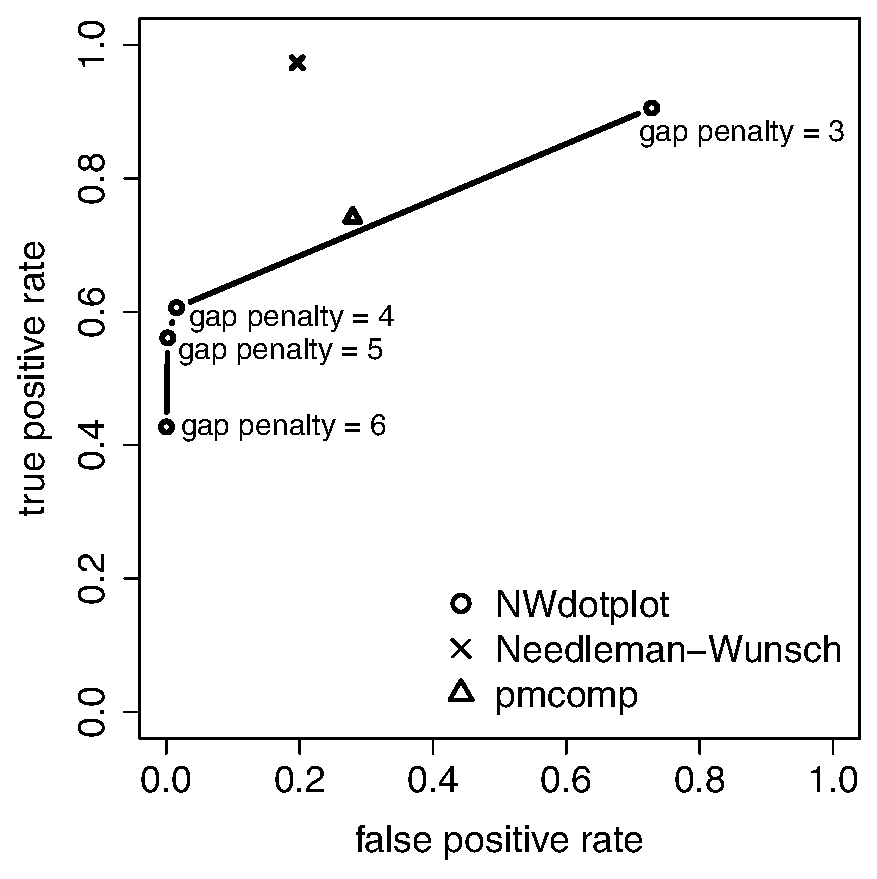
\epsfig{ file = snornal140_roc.eps, width = 0.45\textwidth}}
  \caption{Performance comparison of hierarchical cluster analysis: Degree of
  agreement between the 10 tested Rfam families and the automated clustering
  based on distance scores from \dotaligner{} with different gap penalties,
  Needleman-Wunsch algorithm and \pmcomp{}.}
  \label{fig:roc}
\end{figure}

%dotaligner gap 3
%SP = 0.2719
%SN = 0.9057
%dotaligner gap 4
%SP = 0.9846
%SN = 0.6063
%dotaligner gap 5
%SP = 0.9978
%SN = 0.5609
%dotaligner gap 6
%SP = 0.9997
%SN = 0.4273
%nwseq
%SP = 0.8035
%SN = 0.9735
%%SP = 0.8353
%%SN = 0.9833
%pmcomp
%SP = 0.7204
%SN = 0.7414


\subsection{Comparison with other methods}

\noindent We compare \dotaligner{} with sequence alignments (in-house
implementation of Needleman-Wunsch algorithm with the blastn parameters match
$=$ 2, mismatch $=$ -3 and gap penalty $=$ 5 which are optimized for sequence
identity of 90\%) and the structure alignment tools \pmcomp{} (using default
parameters or larger values for parameter \emph{-D} if the length difference of
two sequences is $>$ 5 bp), \RED{\carna, and \locarna}. Figure \ref{fig:roc}
shows that the sequence aligner (SP $=$ 0.80, SN $=$0.97) performs very well on
our benchmark set with a very high sensitivity which is most likely due to the
fact that the input sequences have some degree of sequence information.
\pmcomp{} (SP $=$ 0.72, SN $=$ 0.74) performed with a medium sensitivity and
specificity. With \dotaligner{} we are able to find very well defined clusters (SP
$=$ 0.99), however, at the cost of sensitivity (SN $=$ 0.61), see Figure
\ref{fig:dotaligner_g4_cluster}.

\begin{figure*}[!ht]
  \centering
  {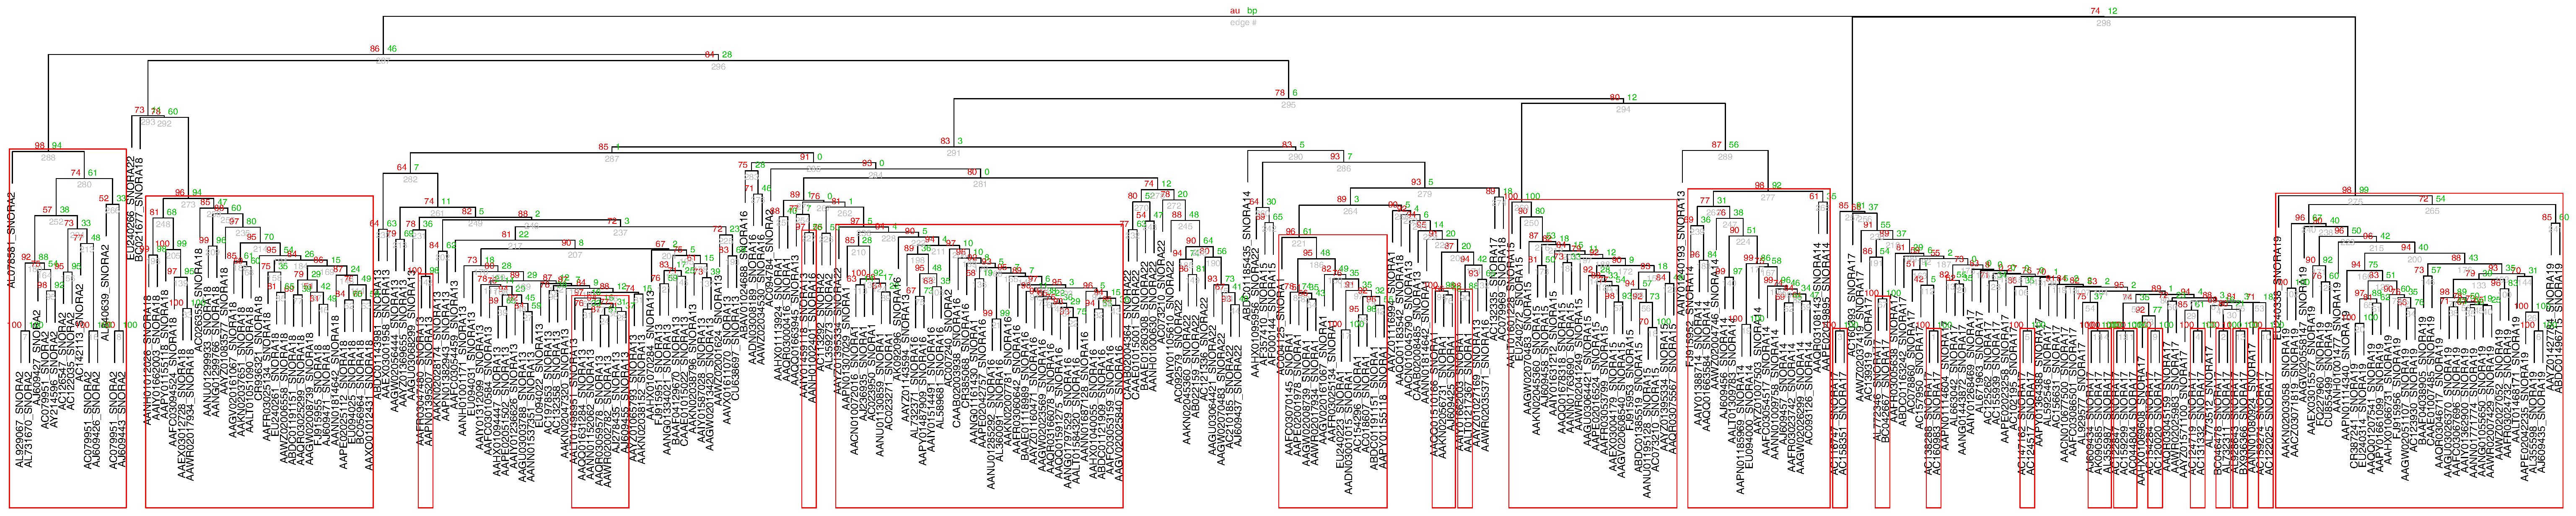
\epsfig{file = snornal140_dotaligner_g4_bootstrap1000.eps, width = 1\textwidth}}
  \caption{Automated hierarchical clustering of 300 sequences from 10 H/ACA
  snoRNA families. The dissimilarity matrix was calculated through \dotaligner{}
  with gap penalty 4. The clustering was conducted by the R-package \pvclust{}
  with multiscale bootstrap resampling with number of bootstrap 1000. We define
  clusters (red rectangles) as Approximately Unbiased (AU) \textit{p}-values $>$
  0.95 rejecting the hypothesis that ``the cluster does not exist`` with
  significance level 0.05.}
  \label{fig:dotaligner_g4_cluster}
\end{figure*}


\subsection{Clustering methodology} 

\noindent The reliability of our pairwise structure alignment algorithm at
clustering homologous RNA structures was tested on a curated database of RNA
structure families (cf RFAM). This enables both qualitative and quantitative
performance evaluation using a gold-standard reference. We compared
\texttt{DotAligner} to other RNA structure alignment and clustering tools using
the following framework: 

\begin{enumerate}
\item Generate dissimilarity matrix $dM_A$ from ${n(n-1)}\over{2}$ pairwise structure comparisons with each algorithm
\item Hierarchical clustering of RNA secondary structures and significance testing with \pvclust{} (Suzuki R and Shimodaira H. Bioinformatics 2006).
\item Generate dissimilarity matrix $dM_R$ from scoring metric of (1.) from curated RFAM alignments (constrained alignment). 
\item Calculate the correlation coefficient between $dM_A$ and $dM_R$ using the Mantel correlation statistic (the cross-product between the standardised distances). 
\end{enumerate}

Benchmarking was performed on both complete RNA structures (global alignment) and randomly selected subsequences (local alignment) for various RFAM families, as described below. \\


\subsection{Benchmark data generation} 

xx RNA families were manually selected from the seed alignments of RFAM 11 (REF). \textit{How should we limit the mean pairwise identity? All structures must be within a given range and perform several independent comparisons, i.e. one per SeqID range? Then compare the individual SeqID ranges to a sample of variable SeqIDs (without selection)?}\\

We employed the BuildRfamBenchmark JAVA program from (Smith M et al. NAR 2013) to generate the sample alignments for the RFAM entries listed in TableXX. The tRNA sample includes special tRNAs, like ser-tRNA with a 5th hairpin to see how the latter gets clustered by the algorithms. \\

%###########  TABLE XX  ############
\begin{tabular}{|c|c|c|}
\hline 
\textbf{RFAM ID} & \textbf{RNA class} & \textbf{average length} \\ 
\hline 
• & 5s rRNA & • \\ 
• & SRP & • \\ 
• & tRNA & • \\ 
• & HaCa snoRNA & • \\ 
• & pre-miRNA & • \\ 
\hline 
\end{tabular} 
%###################################


\subsection{Complete RFAM sequences}

Global alignment. More emphasis on quantitative clustering, accuracy, and correlation with control. 


\subsection{Fragmented RFAM sequences} 

Local alignment, simulating genomic screens. More emphasis on qualitative clustering



\section{\uppercase{Discussion}}

\noindent We plan to integrate the proposed method in a pipeline that screens
regions of interest for structured RNA domains in a collection of RNA molecules.
The pipeline may comprise window based thermodynamic folding, \eg{} by
\rnaplfold{} \cite{Bernhart:Hofacker:Stadler:Local_RNA_base:2006}, the
identification of regions of high intra-molecular binding probabilities, \eg{}
\rnalocal{} \cite{Dotu19908358}, followed by the presented alignment tool
\dotaligner. The identification of local structural potential is necessary because
\dotaligner{} finds only semi-local alignments, meaning the heuristic in the first
step of the algorithm gives global alignment, whereas the second step provides a
final local alignment. 

\dotaligner{} can also be extended for multiple alignments, similar to the strategy
implemented in \pmmulti{} \cite{Hofacker15073017}, and the generation of
phylogenetic trees. This may replace or support the hierarchical clustering
approach used here. In addition, both may serve as input for RNA secondary
structure predictors, such as \petfold{} \cite{Seemann2008} unifying
thermodynamic and evolutionary information. 

The first step of the algorithm could also implement local alignments. In this
case, however, the input basepair probabilities should be calculated in a
sliding-window approach, such as provided by \rnaplfold.  Then step 2 has to
find the best local alignment of local pairwise alignments from step 1 where the
paired bases are overlapping.  The search for overlapping local alignments from
step 1 will increase the running time exponentially, but local alignments may
improve the boundaries of common structured RNA domains.


\section*{\uppercase{Acknowledgements}}

\noindent I thank the Carlsberg foundation for my travel grant. Sk\aa l!


\vfill
\bibliographystyle{apalike}
{\small
\bibliography{dotaligner}}


\vfill
\end{document}

